\documentclass{standalone}
\usepackage{tikz}
\usetikzlibrary{patterns, positioning}


\begin{document}
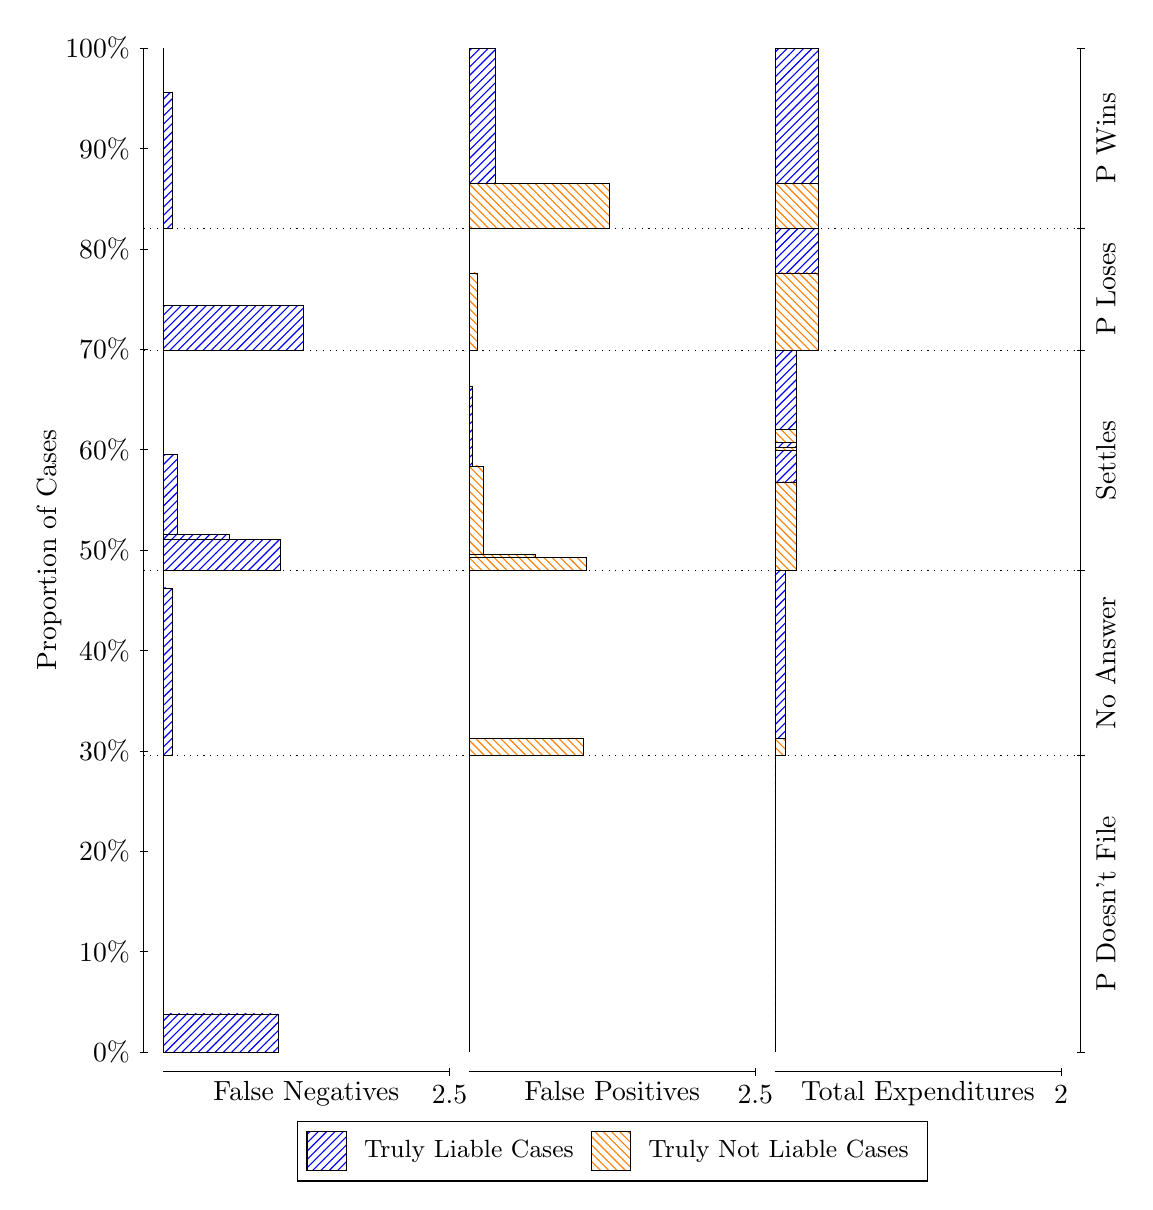
\begin{tikzpicture}
\draw[black, very thin] (1.5,1.75) -- (1.5,14.5);
\node[rotate=90, text=black, anchor=center] at (0.3, 8.125) {Proportion of Cases};
\draw[black, very thin] (1.45,1.75) -- (1.55,1.75);
\node[text=black, anchor=east] at (1.45, 1.75) {0\%};
\draw[black, very thin] (1.45,3.025) -- (1.55,3.025);
\node[text=black, anchor=east] at (1.45, 3.025) {10\%};
\draw[black, very thin] (1.45,4.3) -- (1.55,4.3);
\node[text=black, anchor=east] at (1.45, 4.3) {20\%};
\draw[black, very thin] (1.45,5.575) -- (1.55,5.575);
\node[text=black, anchor=east] at (1.45, 5.575) {30\%};
\draw[black, very thin] (1.45,6.85) -- (1.55,6.85);
\node[text=black, anchor=east] at (1.45, 6.85) {40\%};
\draw[black, very thin] (1.45,8.125) -- (1.55,8.125);
\node[text=black, anchor=east] at (1.45, 8.125) {50\%};
\draw[black, very thin] (1.45,9.4) -- (1.55,9.4);
\node[text=black, anchor=east] at (1.45, 9.4) {60\%};
\draw[black, very thin] (1.45,10.675) -- (1.55,10.675);
\node[text=black, anchor=east] at (1.45, 10.675) {70\%};
\draw[black, very thin] (1.45,11.95) -- (1.55,11.95);
\node[text=black, anchor=east] at (1.45, 11.95) {80\%};
\draw[black, very thin] (1.45,13.225) -- (1.55,13.225);
\node[text=black, anchor=east] at (1.45, 13.225) {90\%};
\draw[black, very thin] (1.45,14.5) -- (1.55,14.5);
\node[text=black, anchor=east] at (1.45, 14.5) {100\%};

\draw[black, very thin] (13.4,1.75) -- (13.4,14.5);
\draw[black, very thin] (13.35,1.75) -- (13.45,1.75);
\node[anchor=west] at (13.35, 1.75) {};
\draw[black, very thin] (13.35,5.5119) -- (13.45,5.5119);
\node[anchor=west] at (13.35, 5.5119) {};
\draw[black, very thin] (13.35,7.8664) -- (13.45,7.8664);
\node[anchor=west] at (13.35, 7.8664) {};
\draw[black, very thin] (13.35,10.664) -- (13.45,10.664);
\node[anchor=west] at (13.35, 10.664) {};
\draw[black, very thin] (13.35,12.213) -- (13.45,12.213);
\node[anchor=west] at (13.35, 12.213) {};
\draw[black, very thin] (13.35,14.5) -- (13.45,14.5);
\node[anchor=west] at (13.35, 14.5) {};

\draw[black, very thin, pattern color=blue, pattern=north east lines] (1.75,1.75) rectangle (3.2033,2.2345);
\draw[black, very thin, pattern color=orange, pattern=north west lines] (1.75,2.2345) rectangle (1.75,5.5119);
\draw[black, very thin, pattern color=blue, pattern=north east lines] (1.75,5.5119) rectangle (1.859,7.6446);
\draw[black, very thin, pattern color=orange, pattern=north west lines] (1.75,7.6446) rectangle (1.75,7.8664);
\draw[black, very thin, pattern color=blue, pattern=north east lines] (1.75,7.8664) rectangle (3.2397,8.2645);
\draw[black, very thin, pattern color=blue, pattern=north east lines] (1.75,8.2645) rectangle (2.5857,8.3268);
\draw[black, very thin, pattern color=blue, pattern=north east lines] (1.75,8.3268) rectangle (1.9317,9.3368);
\draw[black, very thin, pattern color=orange, pattern=north west lines] (1.75,9.3368) rectangle (1.75,10.664);
\draw[black, very thin, pattern color=blue, pattern=north east lines] (1.75,10.664) rectangle (3.5303,11.233);
\draw[black, very thin, pattern color=orange, pattern=north west lines] (1.75,11.233) rectangle (1.75,12.213);
\draw[black, very thin, pattern color=blue, pattern=north east lines] (1.75,12.213) rectangle (1.859,13.932);
\draw[black, very thin, pattern color=orange, pattern=north west lines] (1.75,13.932) rectangle (1.75,14.5);
\draw[black, very thin, pattern color=orange, pattern=north west lines] (5.6333,1.75) rectangle (5.6333,5.0274);
\draw[black, very thin, pattern color=blue, pattern=north east lines] (5.6333,5.0274) rectangle (5.6333,5.5119);
\draw[black, very thin, pattern color=orange, pattern=north west lines] (5.6333,5.5119) rectangle (7.0867,5.7336);
\draw[black, very thin, pattern color=blue, pattern=north east lines] (5.6333,5.7336) rectangle (5.6333,7.8664);
\draw[black, very thin, pattern color=orange, pattern=north west lines] (5.6333,7.8664) rectangle (7.123,8.0329);
\draw[black, very thin, pattern color=orange, pattern=north west lines] (5.6333,8.0329) rectangle (6.469,8.0696);
\draw[black, very thin, pattern color=orange, pattern=north west lines] (5.6333,8.0696) rectangle (5.815,9.1939);
\draw[black, very thin, pattern color=blue, pattern=north east lines] (5.6333,9.1939) rectangle (5.6697,10.204);
\draw[black, very thin, pattern color=blue, pattern=north east lines] (5.6333,10.204) rectangle (5.6333,10.664);
\draw[black, very thin, pattern color=orange, pattern=north west lines] (5.6333,10.664) rectangle (5.7423,11.644);
\draw[black, very thin, pattern color=blue, pattern=north east lines] (5.6333,11.644) rectangle (5.6333,12.213);
\draw[black, very thin, pattern color=orange, pattern=north west lines] (5.6333,12.213) rectangle (7.4137,12.782);
\draw[black, very thin, pattern color=blue, pattern=north east lines] (5.6333,12.782) rectangle (5.9603,14.5);
\draw[black, very thin, pattern color=orange, pattern=north west lines] (9.5167,1.75) rectangle (9.5167,5.0274);
\draw[black, very thin, pattern color=blue, pattern=north east lines] (9.5167,5.0274) rectangle (9.5167,5.5119);
\draw[black, very thin, pattern color=orange, pattern=north west lines] (9.5167,5.5119) rectangle (9.6529,5.7336);
\draw[black, very thin, pattern color=blue, pattern=north east lines] (9.5167,5.7336) rectangle (9.6529,7.8664);
\draw[black, very thin, pattern color=orange, pattern=north west lines] (9.5167,7.8664) rectangle (9.7892,8.9907);
\draw[black, very thin, pattern color=blue, pattern=north east lines] (9.5167,8.9907) rectangle (9.7892,9.3888);
\draw[black, very thin, pattern color=orange, pattern=north west lines] (9.5167,9.3888) rectangle (9.7892,9.4255);
\draw[black, very thin, pattern color=blue, pattern=north east lines] (9.5167,9.4255) rectangle (9.7892,9.4879);
\draw[black, very thin, pattern color=orange, pattern=north west lines] (9.5167,9.4879) rectangle (9.7892,9.6544);
\draw[black, very thin, pattern color=blue, pattern=north east lines] (9.5167,9.6544) rectangle (9.7892,10.664);
\draw[black, very thin, pattern color=orange, pattern=north west lines] (9.5167,10.664) rectangle (10.062,11.644);
\draw[black, very thin, pattern color=blue, pattern=north east lines] (9.5167,11.644) rectangle (10.062,12.213);
\draw[black, very thin, pattern color=orange, pattern=north west lines] (9.5167,12.213) rectangle (10.062,12.782);
\draw[black, very thin, pattern color=blue, pattern=north east lines] (9.5167,12.782) rectangle (10.062,14.5);
\draw[black, dotted] (1.5,5.5119) -- (13.4,5.5119);
\draw[black, dotted] (1.5,7.8664) -- (13.4,7.8664);
\draw[black, dotted] (1.5,10.664) -- (13.4,10.664);
\draw[black, dotted] (1.5,12.213) -- (13.4,12.213);
\draw[black, very thin] (1.75,1.5) -- (5.3833,1.5);
\node[text=black, anchor=north] at (3.5667, 1.5) {False Negatives};
\draw[black, very thin] (5.3833,1.45) -- (5.3833,1.55);
\node[text=black, anchor=north] at (5.3833, 1.45) {2.5};

\draw[black, very thin] (5.6333,1.5) -- (9.2667,1.5);
\node[text=black, anchor=north] at (7.45, 1.5) {False Positives};
\draw[black, very thin] (9.2667,1.45) -- (9.2667,1.55);
\node[text=black, anchor=north] at (9.2667, 1.45) {2.5};

\draw[black, very thin] (9.5167,1.5) -- (13.15,1.5);
\node[text=black, anchor=north] at (11.333, 1.5) {Total Expenditures};
\draw[black, very thin] (13.15,1.45) -- (13.15,1.55);
\node[text=black, anchor=north] at (13.15, 1.45) {2};

\node[text=black, centered, rotate=90] at (13.72, 3.6309) {P Doesn't File};
\node[text=black, centered, rotate=90] at (13.72, 6.6891) {No Answer};
\node[text=black, centered, rotate=90] at (13.72, 9.2654) {Settles};
\node[text=black, centered, rotate=90] at (13.72, 11.439) {P Loses};
\node[text=black, centered, rotate=90] at (13.72, 13.357) {P Wins};

\draw (7.449999999999999,1.5) node[draw=none] (baseCoordinate) {};
\begin{scope}[align=center]
        \matrix[scale=0.5, draw=black, below=0.5cm of baseCoordinate, nodes={draw}, column sep=0.1cm]{
            \node[rectangle, draw, minimum width=0.5cm, minimum height=0.5cm, pattern color=blue, pattern=north east lines] {}; &
            \node[draw=none, font=\small, text=black] (B) {Truly Liable Cases}; &
            \node[rectangle, draw, minimum width=0.5cm, minimum height=0.5cm, pattern color=orange, pattern=north west lines] {}; &
            \node[draw=none, font=\small, text=black] (B) {Truly Not Liable Cases}; \\
            };
\end{scope}

\end{tikzpicture}
\end{document}